\documentclass[tikz,border=10pt]{standalone}
% Only base TikZ is needed; no extra libraries.
\begin{document}
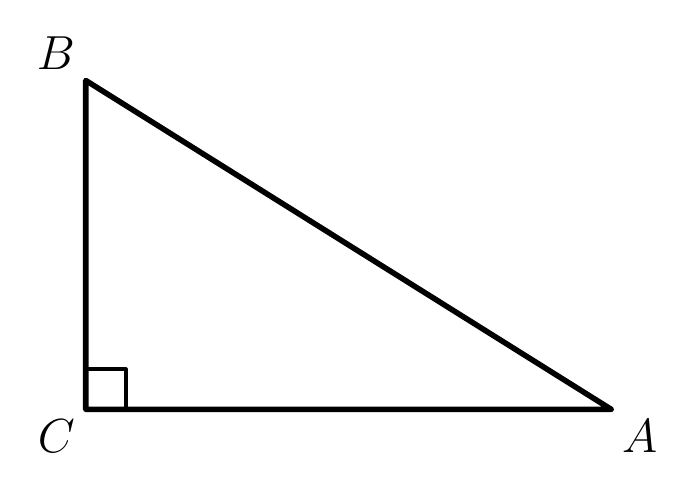
\begin{tikzpicture}[line width=1.2pt, line join=round]
  % Coordinates: origin at C, s = 0.021277 cm/px (longest side = 8 cm), y flipped
  \coordinate (C) at (0,0);
  \coordinate (A) at (6.672,0);     % A: (381.6-68)*s, 0
  \coordinate (B) at (0,4.176);     % B: 0, (262-65.75)*s

  % Triangle sides: thick (~2pt) to match original ~3px stroke
  \draw[line width=2pt] (A) -- (B) -- (C) -- cycle;

  % Right-angle mark at C, side ~0.51 cm (about 12% larger), inside the triangle
  \draw (0.51,0) -- (0.51,0.51) -- (0,0.51);

  % Labels
  \node[font=\fontsize{17.5}{21}\selectfont, anchor=north west] at (A) {$A$};
  \node[font=\fontsize{17.5}{21}\selectfont, anchor=south east] at (B) {$B$};
  \node[font=\fontsize{17.5}{21}\selectfont, anchor=north east] at (C) {$C$};
\end{tikzpicture}
\end{document}